% A short deck on the unpaired PYTHIA -> JEWEL jet translation pilot
% (FLOW_NOTES.md, "PYTHIA -> JEWEL translation pilot"; the detailed appendix is
% translation_appendix.pdf). Numbers: docs/flow/translation/*.csv
% (translation_report.py); figures: docs/flow/translation/deck_*.png
% (translation_deck_figs.py). Build:
%   cd docs/flow/translation/slides && ~/pyext/tectonic_env/bin/tectonic translation_deck.tex
\documentclass[aspectratio=169,10pt]{beamer}
\usetheme{default}
\setbeamertemplate{navigation symbols}{}

\usepackage{booktabs}
\usepackage{graphicx}
\usepackage{xcolor}
\usepackage{tikz}
\usetikzlibrary{positioning,arrows.meta}
\graphicspath{{../}}

% ink and series colours of the figures (blue / orange: colour-vision safe)
\definecolor{ink}{HTML}{0B0B0B}
\definecolor{ink2}{HTML}{52514E}
\definecolor{muted}{HTML}{898781}
\definecolor{rule}{HTML}{E1E0D9}
\definecolor{cOT}{HTML}{2A78D6}
\definecolor{cDSBM}{HTML}{EB6834}
\definecolor{wash}{HTML}{F4F3EF}

\setbeamercolor{normal text}{fg=ink}
\setbeamercolor{frametitle}{fg=ink}
\setbeamercolor{title}{fg=ink}
\setbeamercolor{subtitle}{fg=ink2}
\setbeamercolor{date}{fg=muted}
\setbeamercolor{itemize item}{fg=muted}
\setbeamercolor{itemize subitem}{fg=muted}
\setbeamercolor{enumerate item}{fg=ink2}
\setbeamerfont{frametitle}{size=\Large,series=\bfseries}
\setbeamerfont{title}{size=\LARGE,series=\bfseries}
\setbeamertemplate{itemize items}{\raisebox{0.15em}{\scalebox{0.7}{$\blacksquare$}}}
\setbeamertemplate{itemize subitem}{--}
\setbeamersize{text margin left=1.5em,text margin right=1.5em}
\setbeamertemplate{frametitle}{\vspace{0.6em}\insertframetitle\par\vspace{-0.2em}%
  {\color{rule}\rule{\textwidth}{0.6pt}}}
\setbeamertemplate{footline}{\hfill{\scriptsize\color{muted}%
  \insertframenumber\,/\,\inserttotalframenumber}\hspace{1.5em}\vspace{0.9em}}

% a line key in a series colour, then the name in ink
\newcommand{\keyot}{{\color{cOT}\rule[0.25em]{1.1em}{1.6pt}}\,}
\newcommand{\keyds}{{\color{cDSBM}\rule[0.25em]{0.45em}{1.6pt}\hspace{0.2em}\rule[0.25em]{0.45em}{1.6pt}}\,}
\newcommand{\ot}{\textbf{OT-CFM}}
\newcommand{\dsbm}{\textbf{$\alpha$-DSBM}}
\newcommand{\smallnote}[1]{{\footnotesize\color{ink2}#1\par}}

\title{Turning PYTHIA jets into JEWEL jets\\with flow matching}
\subtitle{An unpaired translation pilot on clean calorimeter jet images}
% \author{}
\date{October 2026}

\begin{document}

% ---------------------------------------------------------------- 1
{\setbeamertemplate{footline}{}
\begin{frame}
\vspace{2.5em}
\titlepage
\vfill
{\footnotesize\color{muted} seed 0, 2 GPU hours per model, 20k held-out jets per sample; full log:
\texttt{FLOW\_NOTES.md}, results: \texttt{docs/flow/translation}\par}
\end{frame}}

% ---------------------------------------------------------------- 2
\begin{frame}{The question}
\begin{columns}[c]
\column{0.53\textwidth}
\large
Can a model trained on \textbf{unpaired} samples map a clean PYTHIA (vacuum) jet to a JEWEL-like
(medium) jet?

\vspace{0.8em}
\normalsize
Two things must hold:
\begin{enumerate}
\item the outputs look like real JEWEL jets, statistically;
\item each output still depends on its own input jet.
\end{enumerate}

\vspace{0.6em}
\smallnote{There is no true JEWEL partner for a PYTHIA jet: any unpaired map is one of many with the same
distributions. So this tests distributions and dependence, not a per-jet medium modification.}
\column{0.47\textwidth}
\centering
\begin{tikzpicture}[font=\footnotesize, every node/.style={inner sep=1pt}]
  \node (in) {
\includegraphics[width=2.0cm]{deck_thumb_in.png}};
  \node[below=2pt of in, text=ink2] {PYTHIA jet};
  \node (out) [right=1.7cm of in] {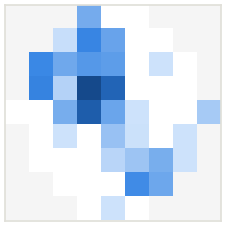
\includegraphics[width=2.0cm]{deck_thumb_out.png}};
  \node[below=2pt of out, text=ink2] {output};
  \draw[-{Stealth[length=6pt]}, line width=1.2pt, cOT] (in) -- node[above=3pt, text=ink] {flow}
    node[below=3pt, text=ink2] {(ODE)} (out);
  \node (jw) [below=1.35cm of out] {
\includegraphics[width=2.0cm]{deck_thumb_jewel.png}};
  \node[below=2pt of jw, text=ink2] {real JEWEL jets};
  \draw[{Stealth[length=5pt]}-{Stealth[length=5pt]}, line width=0.8pt, muted, dashed]
    ([yshift=-14pt]out.south) -- node[right=3pt, text=ink, align=left] {same\\statistics?}
    (jw.north);
  \node[below=1.35cm of in, text=ink2, align=center, text width=2.4cm] {trained on 200k\\PYTHIA + 200k JEWEL
    jets, \textbf{no pairs}};
\end{tikzpicture}
\end{columns}
\end{frame}

% ---------------------------------------------------------------- 3
\begin{frame}{Setup}
\begin{columns}[T]
\column{0.48\textwidth}
\textbf{Data}: clean jet images, no background
\begin{itemize}\setlength\itemsep{0.3em}
\item PYTHIA 2.6M events, JEWEL 870k events
\item the leading R = 0.4 jet ($\ge$ 10 GeV): 53 towers in GeV on a 16 $\times$ 16 grid
\item per sample: 200k training jets, 20k held-out test jets, split by event
\end{itemize}
\vspace{0.6em}
\textbf{Compared with}
\begin{itemize}\setlength\itemsep{0.3em}
\item \dsbm{}: learns its own, random pairing (same network and budget)
\item the PYTHIA jet unchanged; a second JEWEL sample (best possible)
\end{itemize}
\column{0.52\textwidth}
\textbf{Model}: \ot{}, optimal-transport flow matching
\begin{itemize}\setlength\itemsep{0.3em}
\item pair each batch of 256 PYTHIA and 256 JEWEL jets by optimal transport (least change in log energy)
\item learn the velocity along straight lines between pairs (UVCGAN-S network, 32M parameters; 2 hours on
  one A6000)
\item translate a jet by solving the flow ODE: 128 network calls, 6.6 ms per jet
\end{itemize}
\end{columns}
\end{frame}

% ---------------------------------------------------------------- 4
\begin{frame}{The output distributions match JEWEL}
\begin{columns}[c]
\column{0.55\textwidth}
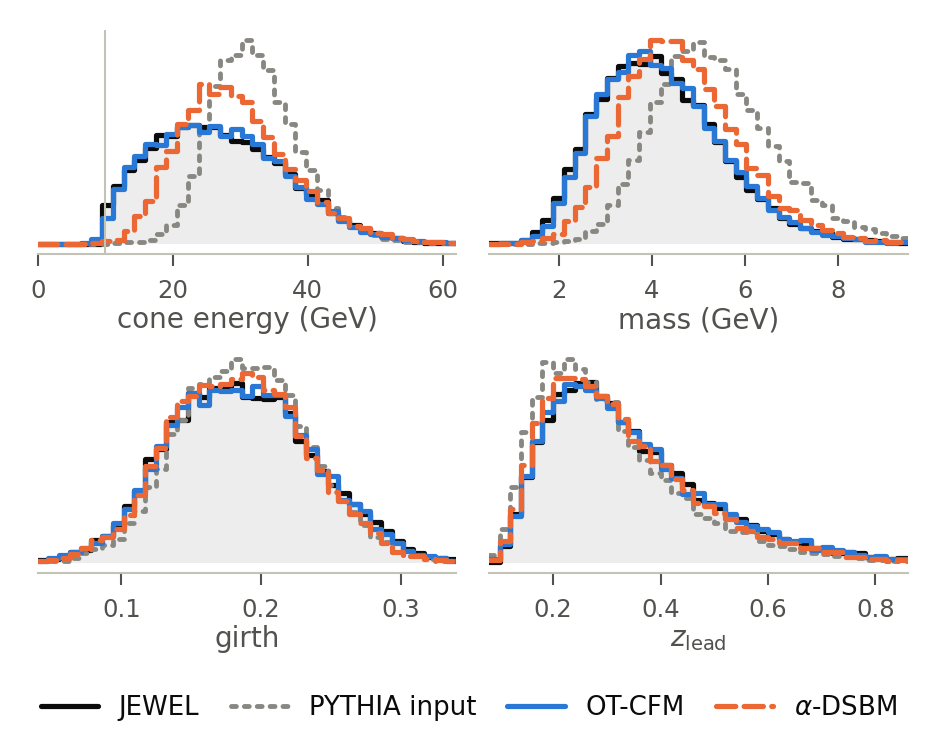
\includegraphics[width=\textwidth]{deck_marginals.png}
\column{0.45\textwidth}
\footnotesize
\setlength{\tabcolsep}{3.5pt}
\begin{tabular}{lrrrr}
\toprule
 & $E$ & mass & girth & $z_\mathrm{lead}$ \\
\midrule
JEWEL vs JEWEL & 0.011 & 0.014 & 0.009 & 0.019 \\
PYTHIA input & 0.55 & 0.88 & 0.10 & 0.23 \\
\keyot OT-CFM & \textbf{0.025} & \textbf{0.021} & \textbf{0.012} & \textbf{0.008} \\
\keyds $\alpha$-DSBM & 0.26 & 0.33 & 0.06 & 0.10 \\
\bottomrule
\end{tabular}
\smallnote{Distance to 20k held-out JEWEL jets (W1 / $\sigma$); lower is better.}

\vspace{0.8em}
\normalsize
\begin{itemize}\setlength\itemsep{0.35em}
\item \ot{} is as close to JEWEL as a second JEWEL sample, within statistical errors; the same holds for
  $p_T^D$, $z_g$, $R_g$ and for jets re-found with anti-$k_T$
\item \dsbm{} closes 51-64\% of the gap
\end{itemize}
\end{columns}
\end{frame}

% ---------------------------------------------------------------- 5
\begin{frame}{Jet shapes at fixed energy are reproduced too}
\begin{center}
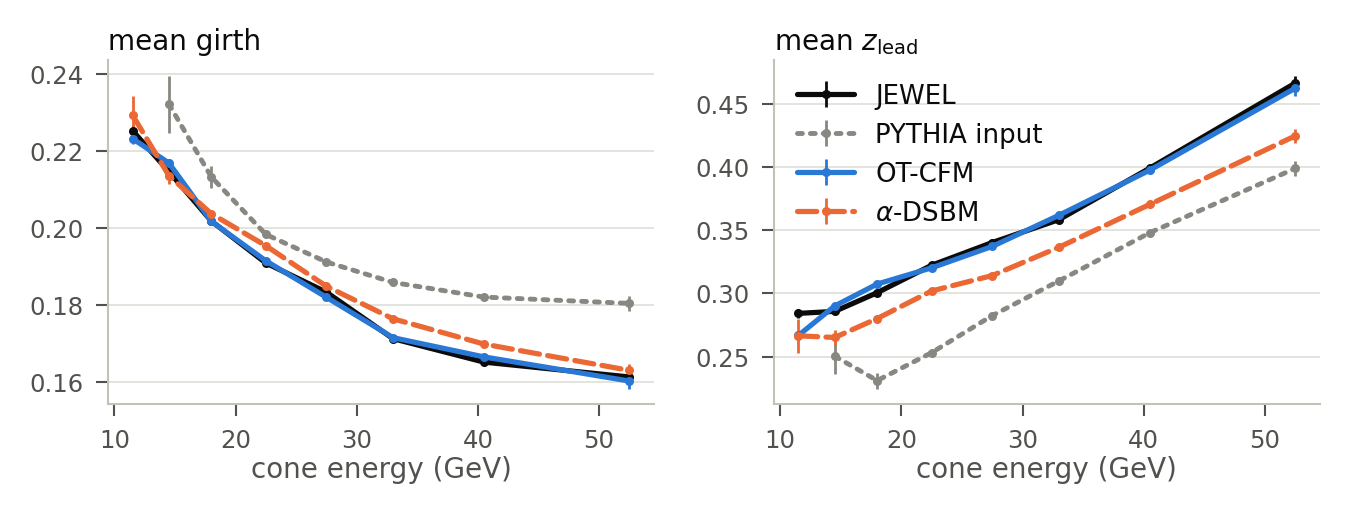
\includegraphics[width=0.8\textwidth]{deck_profiles.png}
\end{center}
\vspace{-0.4em}
\begin{itemize}\setlength\itemsep{0.35em}
\item at the same energy, JEWEL jets are \textbf{narrower} and \textbf{harder} (higher $z_\mathrm{lead}$)
  than PYTHIA jets
\item \ot{} follows both trends in every energy bin; \dsbm{} gets part of the way
\end{itemize}
\end{frame}

% ---------------------------------------------------------------- 6
\begin{frame}{Each output keeps its input jet}
\begin{columns}[c]
\column{0.5\textwidth}
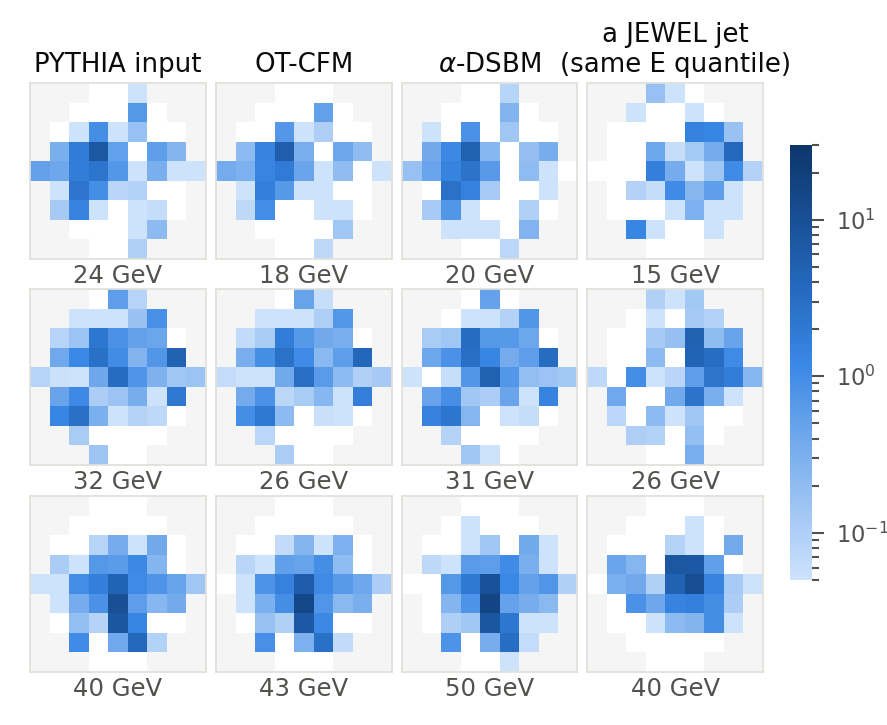
\includegraphics[width=\textwidth]{deck_displays.png}
\column{0.5\textwidth}
\begin{itemize}\setlength\itemsep{0.5em}
\item \ot{}: input-output correlation 0.94 (energy), 0.99 (girth), 0.91 (mass)
\item every output is closer in shape to its own input than to another, random input jet, by
  11$\times$ on average
\item a random JEWEL jet has the right distributions but correlation 0: matching distributions alone
  proves nothing
\item \dsbm{}: 0.80 (energy), 0.98 (girth); two samples of one jet differ more than a sample differs from
  its input
\end{itemize}
\vspace{0.3em}
\smallnote{Fixed held-out inputs (cone-energy quantiles 0.1, 0.5, 0.9). The JEWEL jet is a reference at the
same energy quantile, not a truth.}
\end{columns}
\end{frame}

% ---------------------------------------------------------------- 7
\begin{frame}{Caveat: the energy change mirrors the two samples}
\begin{center}
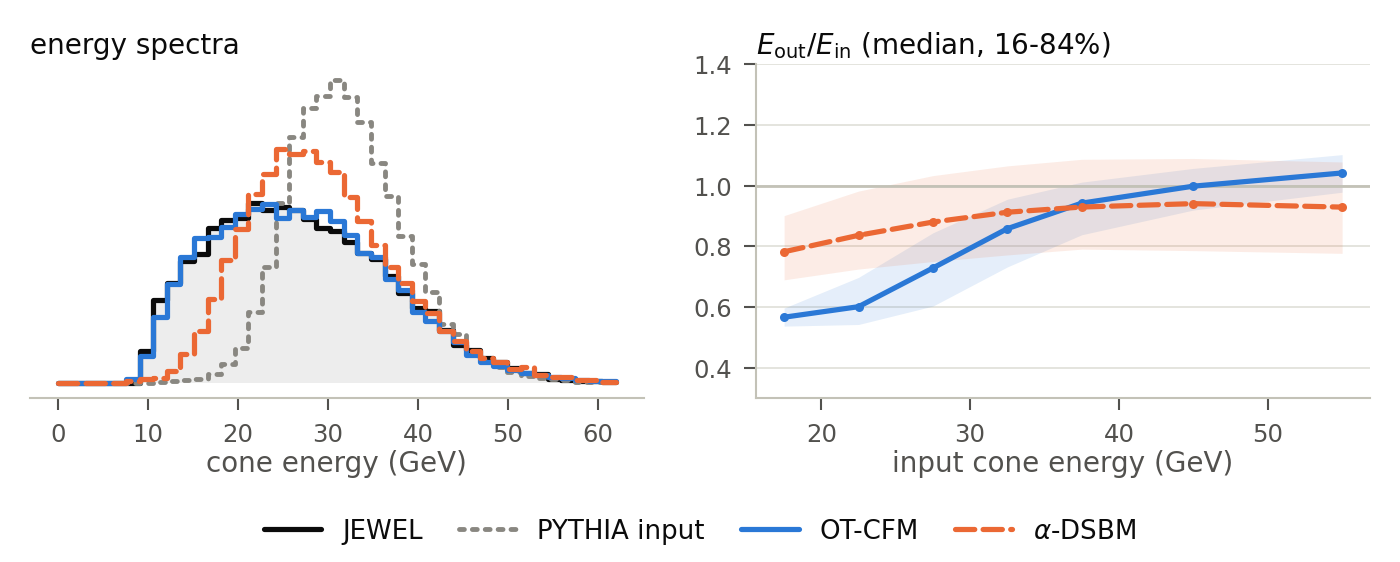
\includegraphics[width=0.82\textwidth]{deck_energy.png}
\end{center}
\vspace{-0.5em}
\begin{itemize}\setlength\itemsep{0.35em}
\item the PYTHIA sample starts near 20 GeV (presumably its generator-level jet requirement); JEWEL
  reaches down to 10 GeV
\item \ot{} lowers 20-25 GeV jets by 40\% and leaves jets above 40 GeV unchanged: a map between two
  differently selected samples, not a quenching mechanism
\end{itemize}
\end{frame}

% ---------------------------------------------------------------- 8
\begin{frame}{Summary}
\begin{columns}[T]
\column{0.5\textwidth}
\textbf{Shown}
\begin{itemize}\setlength\itemsep{0.4em}
\item trained without pairs in 2 GPU hours, \ot{} produces jets statistically indistinguishable from
  held-out JEWEL: 7 observables, their energy dependence, re-found jets
\item each output stays tied to its input (correlations 0.91-0.99)
\item \dsbm{}, same budget: about half way
\end{itemize}
\column{0.5\textwidth}
\textbf{Not shown}
\begin{itemize}\setlength\itemsep{0.4em}
\item a per-jet medium modification: there is no per-jet truth, and optimal transport picks the
  least-change map
\item physics in the energy shift: it reflects how the samples were selected
\item robustness: one seed
\end{itemize}
\end{columns}
\vspace{1.2em}
\colorbox{wash}{\parbox{0.97\linewidth}{\vspace{0.4em}\hspace{0.3em}\textbf{Next:} train two more seeds.
Does the same PYTHIA jet get the same output, not only the same distributions?\vspace{0.4em}}}

\vspace{0.8em}
\smallnote{Practical: the ODE needs 128 network calls (a 4-step solve barely moves the jets); towers
that should be empty get $\sim$0.002 GeV, 0.1\% of the jet energy.}
\end{frame}

\end{document}
